\section{Теоритические сведения}
\[
    f(t) = \frac{A_{0}}{2} + \sum_{n=1}^{\infty} A_{n}\cos(2\pi\nu_{n}t)+B_{n}\sin(2\pi\nu_{n}t)
\]
$\nu_{n} = n\nu_{0}$, $\nu_{0} = 1/T$
\[
    A_{n} = \frac{2}{T}\int_{0}^{T}f(t)\cdot \cos(2\pi\nu_{n}t)dt
\]
\[
    B_{n} = \frac{2}{T}\int_{0}^{T}f(t) \cdot \sin(2\pi\nu_{n}t)dt
\]

\[
    \Delta \nu \cdot \Delta t ~ 1
\]

Методы спектрального анализа можно разделить на цифровые и физические.

Простейший физический метод~--- $RLC$-цепочка. Такой контур отсеивает все чистоты ктроме
близких к резонансной. 

Цифровые методы можно прменить только к низким састотам. 

\begin{figure}[ht!]
    \center{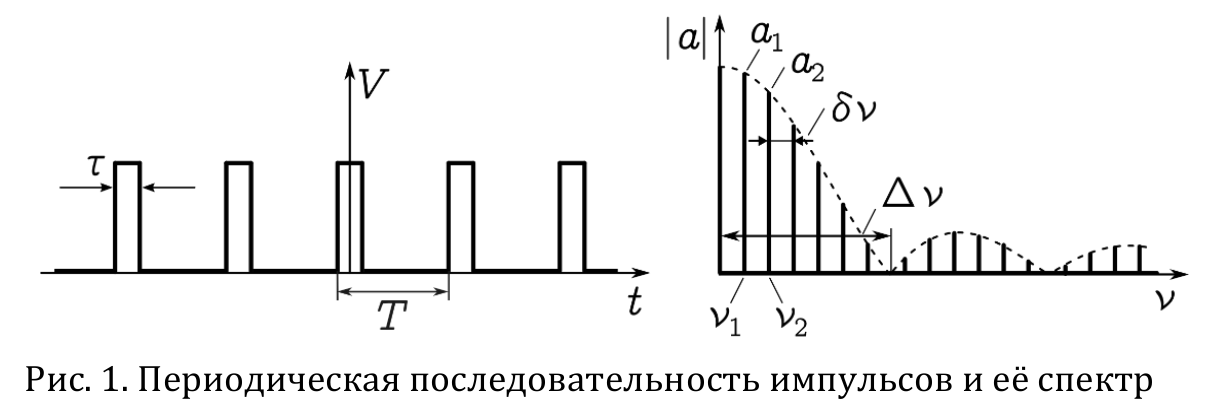
\includegraphics[width=0.8\linewidth]{../img/eq1.png}}
\end{figure}
\begin{figure}[ht!]
    \center{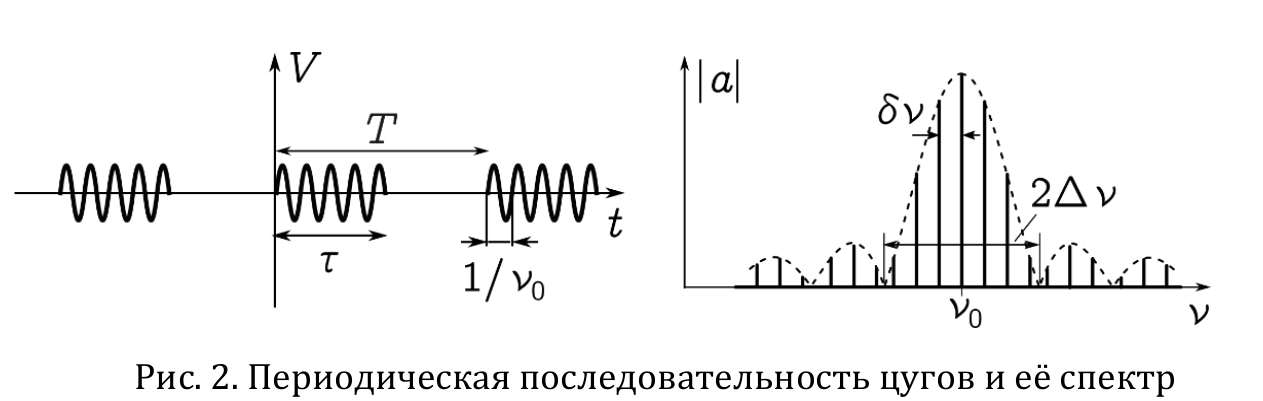
\includegraphics[width=0.8\linewidth]{../img/eq2.png}}
\end{figure}
\begin{figure}[ht!]
    \center{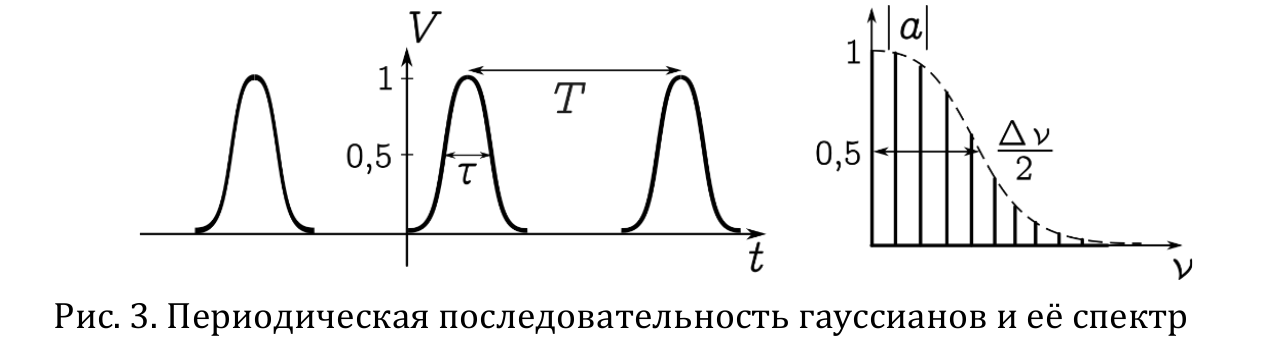
\includegraphics[width=0.8\linewidth]{../img/eq3.png}}
\end{figure}
\begin{figure}[ht!]
    \center{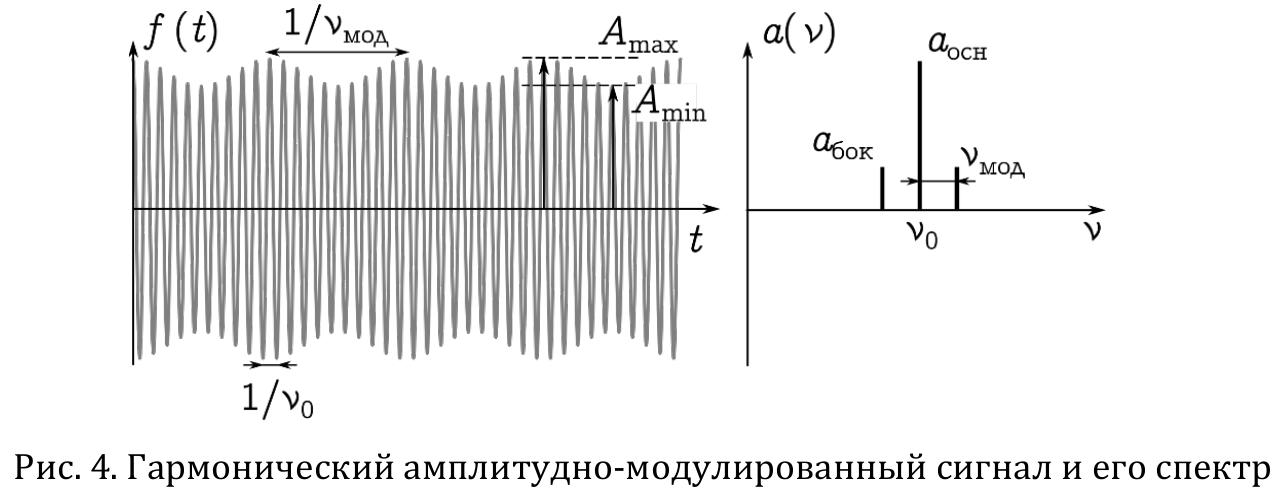
\includegraphics[width=0.8\linewidth]{../img/eq4.png}}
\end{figure}
\begin{figure}[ht!]
    \center{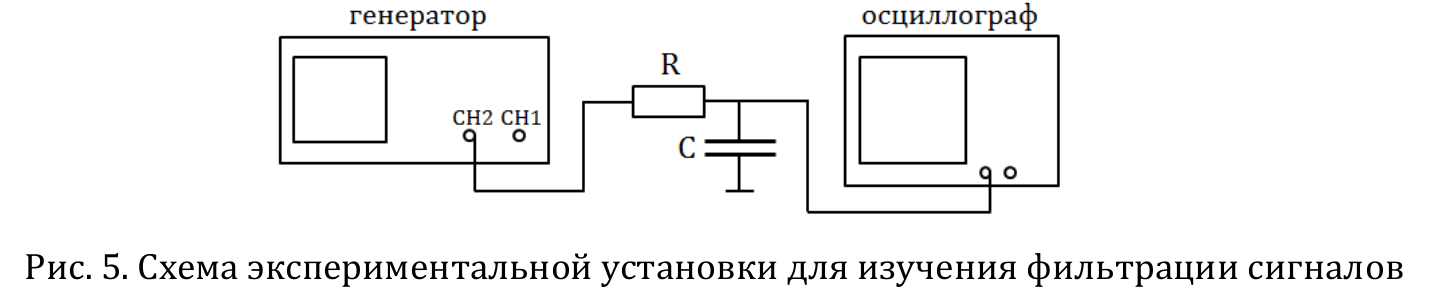
\includegraphics[width=0.8\linewidth]{../img/eq5.png}}
\end{figure}

